\chapter{Конструкторский раздел}
\label{cha:design}

В данном разделе будут представлены схемы алгоритмов, выбранных для решения задачи, и диаграмма классов.

\section{Алгоритм срединных смещений}

Схема алгоритма срединных смещений изображена на рисунке \ref{fig:brown_mov_alg}.

\begin{figure}[ph!]
	\center{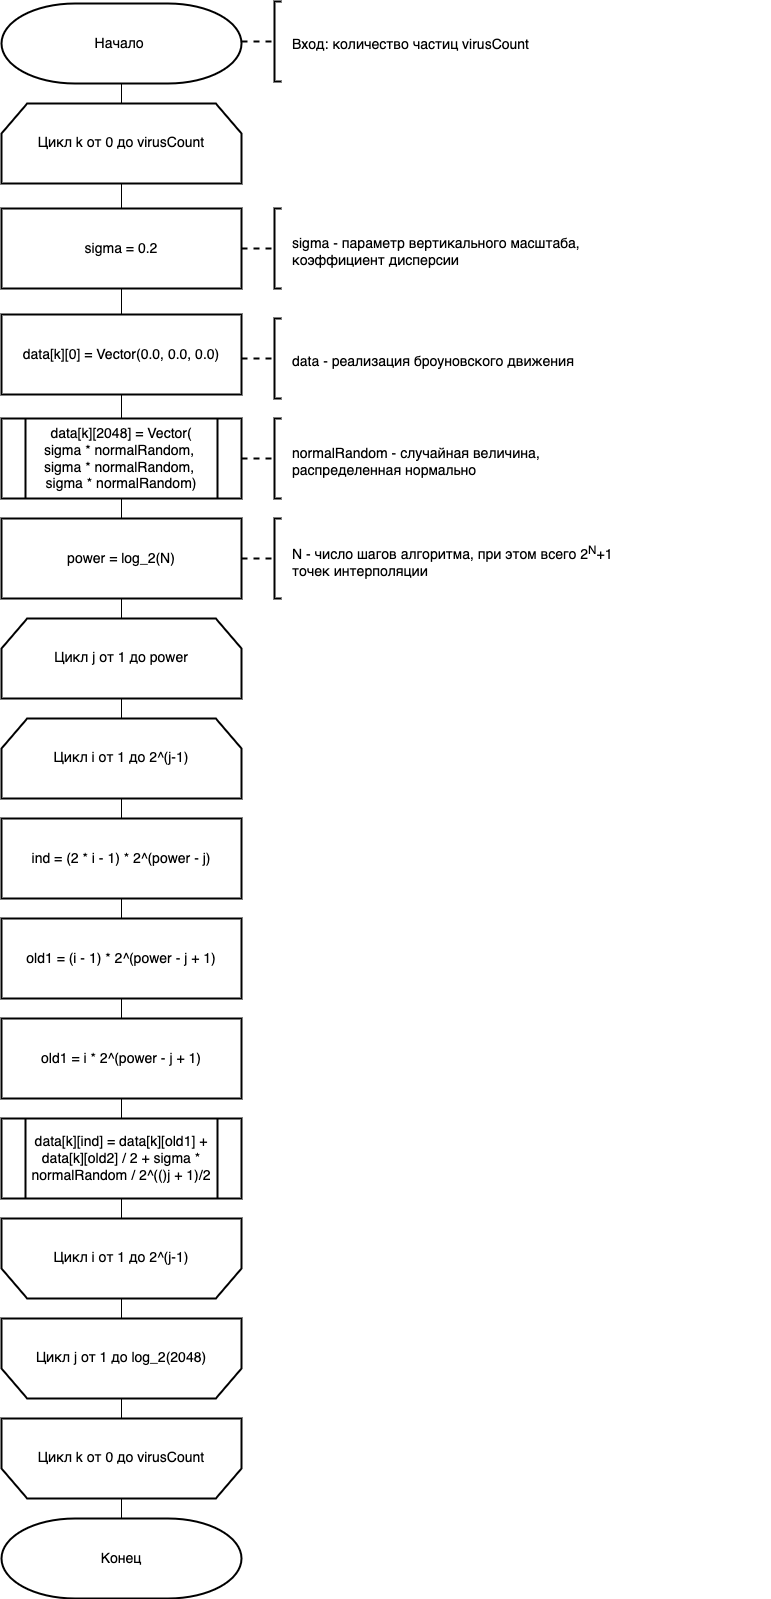
\includegraphics[scale=0.34]{img/brown.png}}
	\caption{Схема алгоритма срединных смещений}
	\label{fig:brown_mov_alg}
\end{figure}

\clearpage

\section{Алгоритмы отрисовки}

Схема алгоритма Z-буфера изображена на рисунке \ref{fig:z_buf_alg}.

\begin{figure}[ph!]
	\center{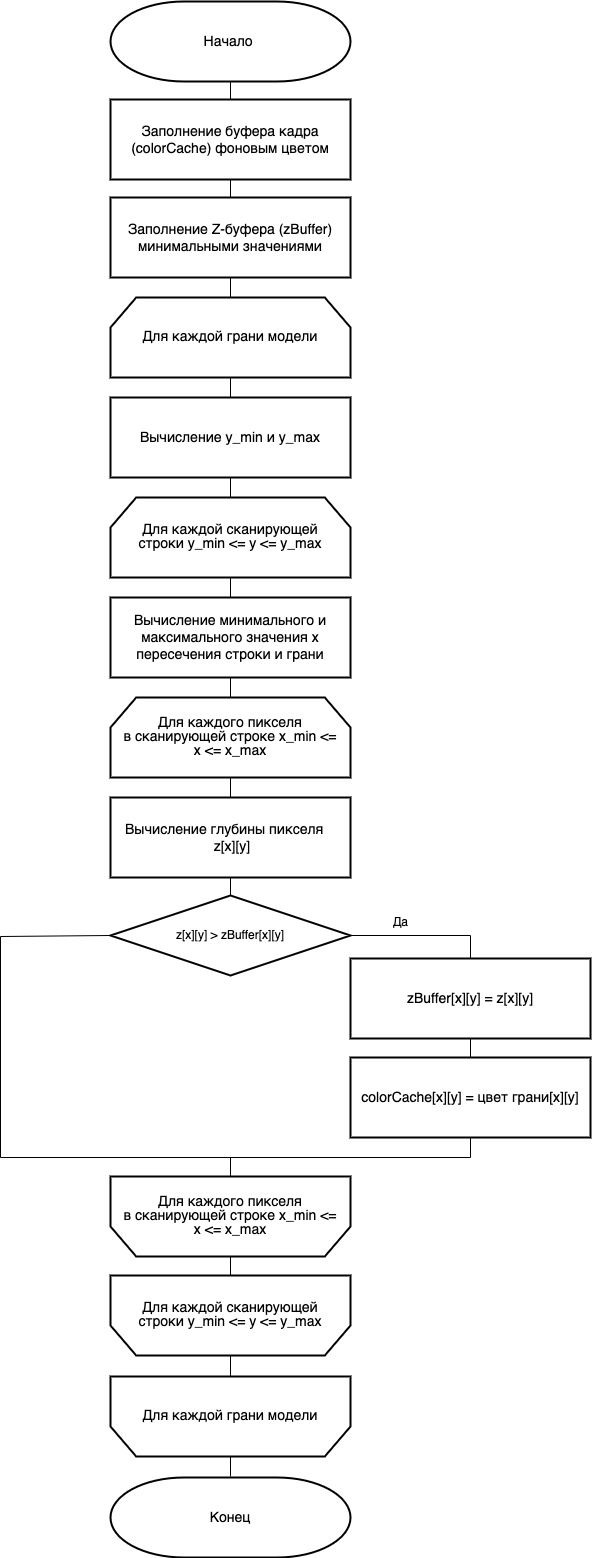
\includegraphics[scale=0.4]{img/z-buffer.png}}
	\caption{Схема алгоритма Z-буфера}
	\label{fig:z_buf_alg}
\end{figure}

\clearpage

Схема алгоритма закраски по Гуро изображена на рисунке \ref{fig:guro_alg}.

\begin{figure}[ph!]
	\center{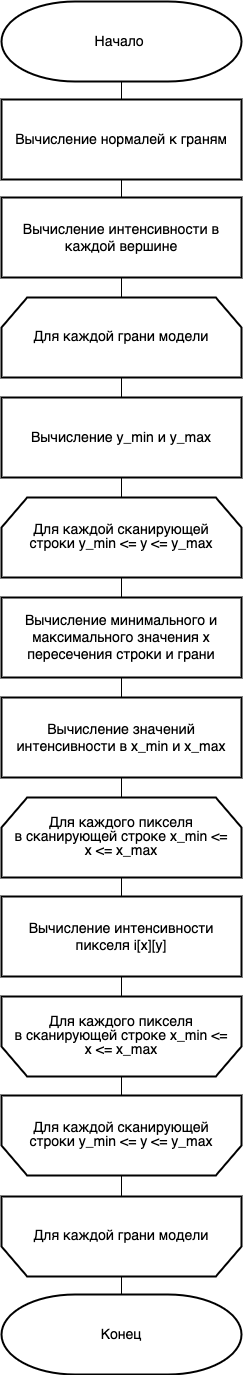
\includegraphics[scale=0.45]{img/guro.png}}
	\caption{Схема алгоритма закраски по Гуро}
	\label{fig:guro_alg}
\end{figure}

\clearpage

\section{Диаграмма классов}

На рисунке \ref{fig:diag_class} представлена диаграмма классов.

\begin{figure}[ph!]
	\center{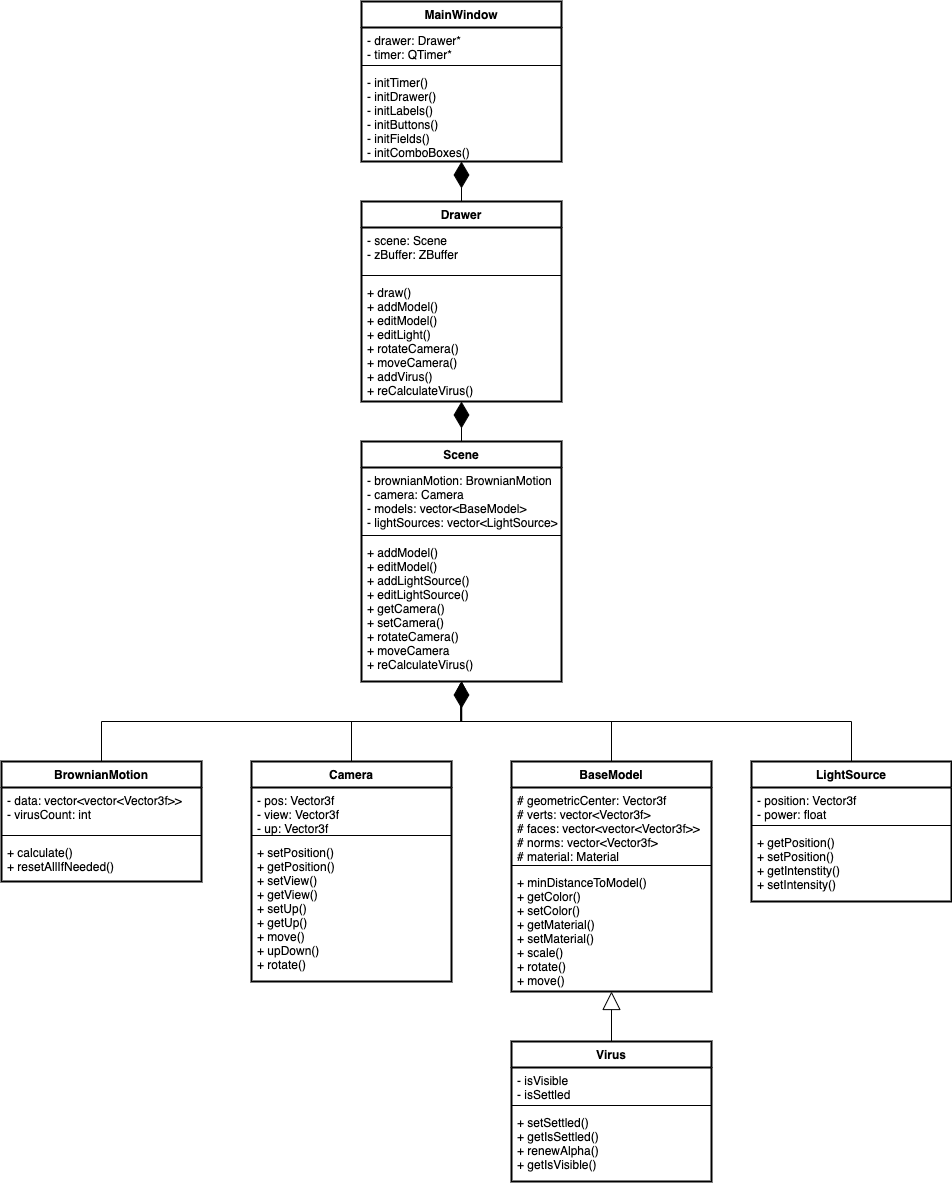
\includegraphics[scale=0.41]{img/classes.png}}
	\caption{Диаграмма классов}
	\label{fig:diag_class}
\end{figure}

\section*{Вывод}
В данном разделе были рассмотрены схемы алгоритмов, использованных при отрисовке сцены, а также диаграмма классов.


